\documentclass[a4paper,twoside,openany]{book}
%twoside Specifies whether double or single sided output should be generated.
%openright/openany Makes chapters begin either only on right hand pages or on the next page available.
\usepackage{geometry}
\geometry{a4paper,top=3cm,bottom=3cm,left=3cm,right=3cm,heightrounded,bindingoffset=1cm}


\usepackage[italian, english]{babel}
\usepackage[T1]{fontenc}
\usepackage{lmodern}
\usepackage{color}
\usepackage{float}
\usepackage{graphicx}
\usepackage{amssymb}
\usepackage{amsmath}
\everymath{\displaystyle}
\usepackage{cancel}
\usepackage{booktabs}
\usepackage{multirow}
\usepackage{siunitx}
\usepackage{subcaption}
\usepackage{hyperref}
\usepackage{hyphenat}
\usepackage{verbatim}
\usepackage{chemformula}
\usepackage{color}
\definecolor{maroon(html/css)}{rgb}{0.5, 0.0, 0.0}
\usepackage{nicematrix}
\usepackage{rotating}

\begin{document}
	\begin{titlepage}
		\centering
		
\includegraphics[width=0.3\textwidth]{university}\\
		\bigskip
		{\Large
		{\scshape Università degli Studi di Milano Bicocca}\\
		{\scshape Dipartimento di Fisica}\\
		{\scshape "Giuseppe Occhialini"}\\
		\bigskip
		{\scshape Corso di Laurea Magistrale in Fisica}\\}
		Anno Accademico 2024/2025\\
		\bigskip
		{\hfill\vfill{\scshape \Huge{\textcolor{maroon(html/css)}{Electrons Drift}}}\\}
		{\vfill
		\[	\begin{array}{c}
			\mbox{Andrea Baiocco}\\
			\mbox{Giovanni Locatelli}\\
			\mbox{Gabriele Papasodaro}\\
			\mbox{Alberto Sala}
			\end{array}	\]}
	\end{titlepage}

\newpage
\null
\thispagestyle{empty}
\newpage

\pagenumbering{Roman}
\setcounter{page}{1}
\begin{center}\textbf{Summary}\\\end{center}
The experience's aim is to study electron drift velocity through a GEM (Gas Electron Multiplier) by changing the electric potential ($\Delta V$) applied to the various stages of the apparatus. Then based on the results, evaluate the drift of the electrons produce by $\alpha$ source.\\
The goal of the experiment is to study the fusion power in a Tokamak, but this can be complicated because the scattering of neutrons makes it difficult to understand whether the neutron is directed or scattered. In a Tokamak, the reaction DT produce $\gamma$-rays, so it is necessary to have a $\gamma$ detector that does not see neutrons by exploiting the Čerenkov effect. Therefore by playing with the pressure, we can adjust the refractive index. By setting a threshold of 10 MeV, we can have a refractive index for the electron of about 0.1, so Čerenkov radiation is produced.

\begin{figure}[H]
\centering
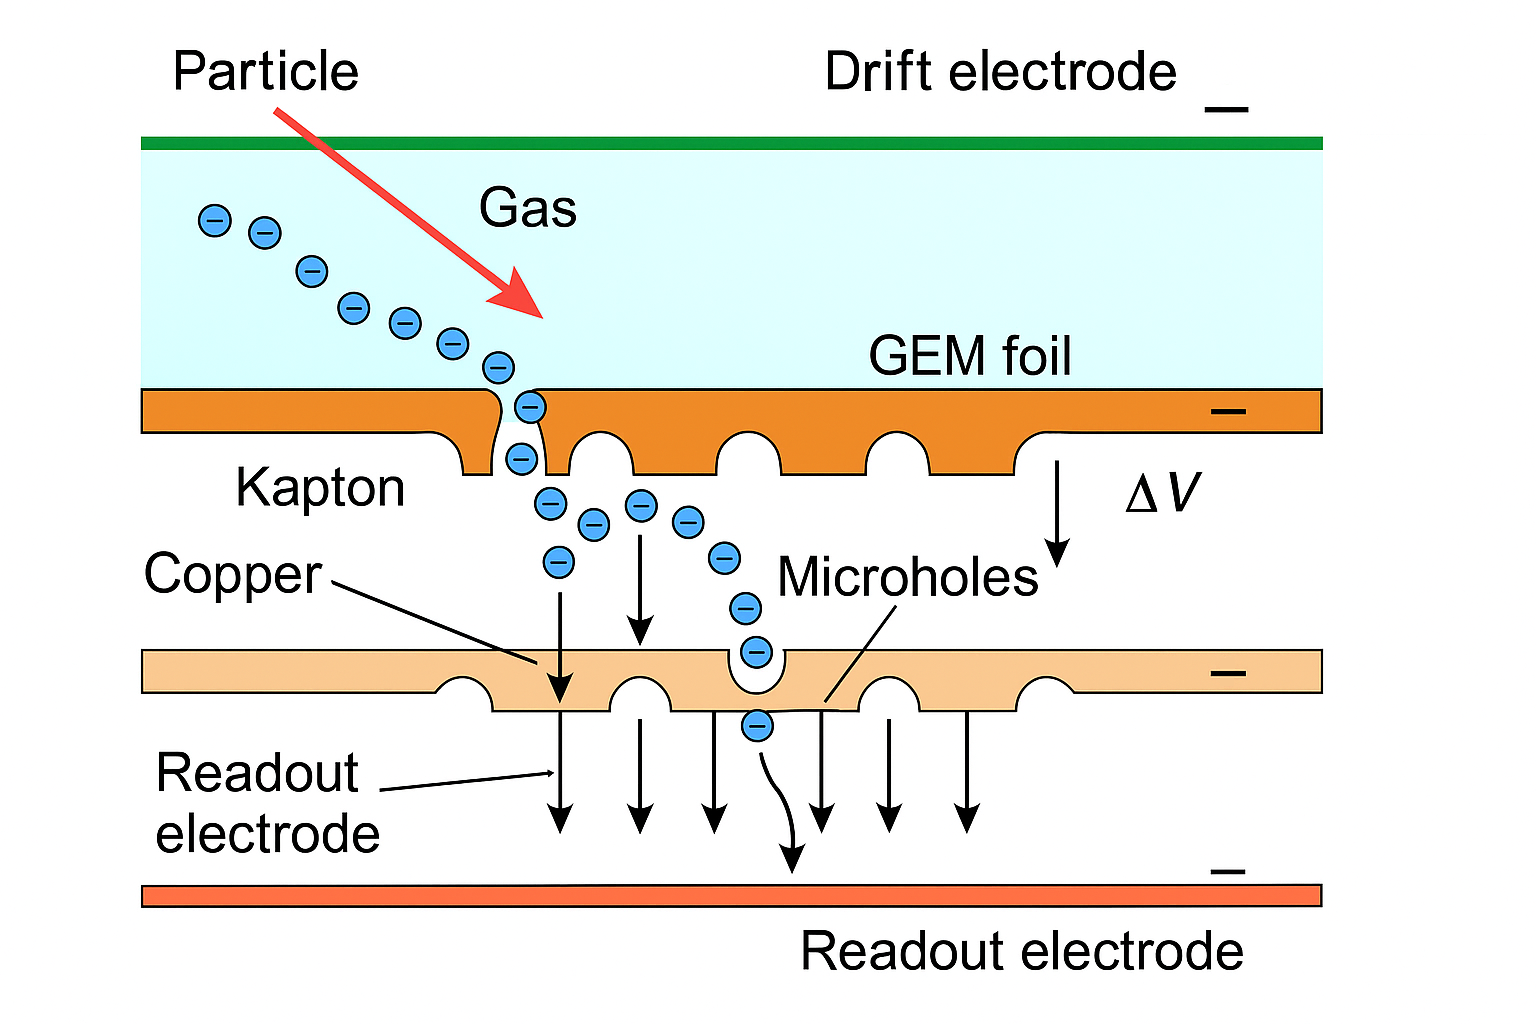
\includegraphics[width=0.4\textwidth, height=0.3\textwidth]{GEM}
\caption{Machine design}
\label{schema}
\end{figure}

The design of the machine in the configurations we studied is very similar, as showed in figure \ref{schema}. The partiularity of our configuration is the polarity of all stages, indeed they  have negative polarity for two reasons:
\begin{enumerate}
\item we are using electrons free charge, that are generate by collisions between $\alpha$ and \ch{N2}, so the stages allow us to direct the particles towards PMT (PhotoMultiplier Tube)
\item allow us to increase the energy of particles in each stages
\end{enumerate}

\begin{figure}[H]
\centering
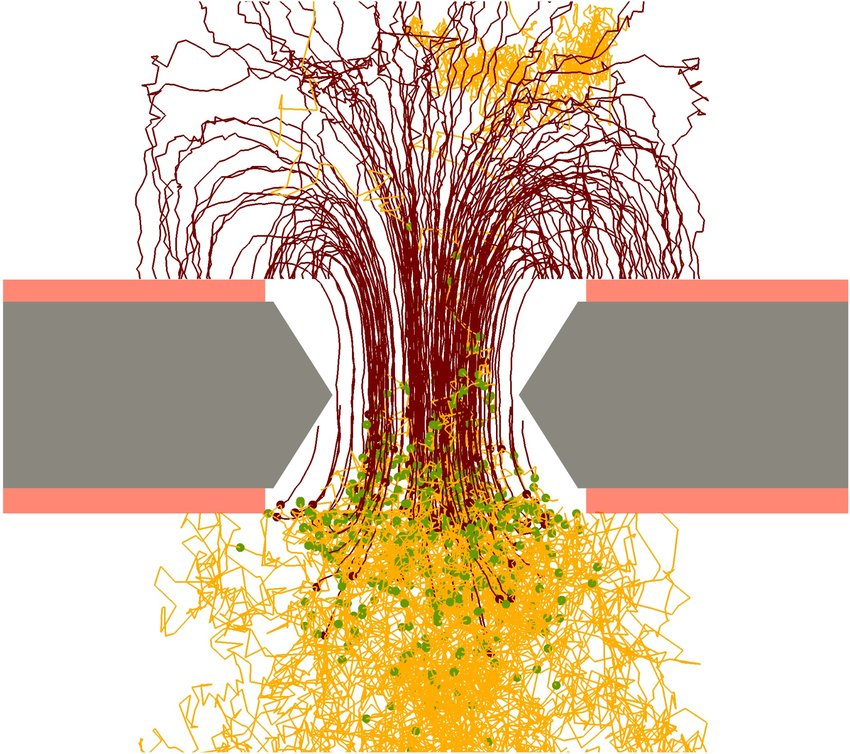
\includegraphics[width=0.3\textwidth]{GEM8}
\caption{Electric field in GEM}
\end{figure}

\newpage
\null
\thispagestyle{empty}
\newpage

\pagenumbering{Roman}
\setcounter{page}{1}
\tableofcontents

\newpage
\null
\thispagestyle{empty}
\newpage

\pagenumbering{arabic}
\setcounter{page}{1}
\chapter{Instruments description}
	\section {Tools list}
\begin{itemize}
\item vacuum chamber
\item pumping system
\item pressure sensor
\item pressure gauge
\item micrometric valve
\item voltage generator
\item $\alpha$ source
\item grid
\item Gas Electron Multiplier (GEM)
\item PhotoMultiplier Tube (PMT)
\item connection BNC
\item\ch{N2}
\item digitizer
\item RC circuit
\item preamplifier
\end{itemize}

	\section{Pumping system, valve...}
The pumping system consists of pipes of various sizes, connections and ties for the connections to the vacuum chamber inside which the cathodes and the GEM are present and finally by a rotary pump.

\begin{figure}[H]
\centering
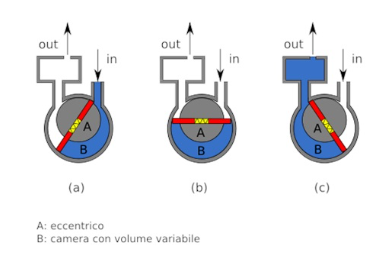
\includegraphics[width=0.3\textwidth]{Rotativa}
\caption{Rotary pump}
\end{figure}

During the entire experience we don't need to work at pressure lower than atmospheric, so the pumping system is used only in the initial phase to clean the chamber from any gaseous impurities. Once the cleaning phase is finished, the system is isolated and connected to a constant flow of nitrogen (\ch{N2}), regulated by the micrometric valve, which is mainly used for two reasons:
\begin{enumerate}
\item convenience, in fact nitrogen is easily available and the cost is not too high
\item the number of Čerenkov neutrons depends on the threshold, therefore since we work for high thresholds (therefore in the ultraviolet region) we need a gas that does not absorb in the UV
\end{enumerate}

	\section{GEM and PMT}
The detector used in the experiment consists of a series assembly of: particle source $\alpha$, Gas Electron Multiplier (GEM) and PhotoMultiplier Tube (PMT).
The signal that we are going to analyze will start instantly at the emission of the $\alpha$, the emitted particles will have energy of about 5$MeV$ according to a Maxwelian distribution. The emitted particle traveling through the gas injected inside the chamber, \ch{N2}, will scintillate through collisions thus producing a cascade of electrons as shown in figure \ref{schema1}.

\begin{figure}[H]
\centering
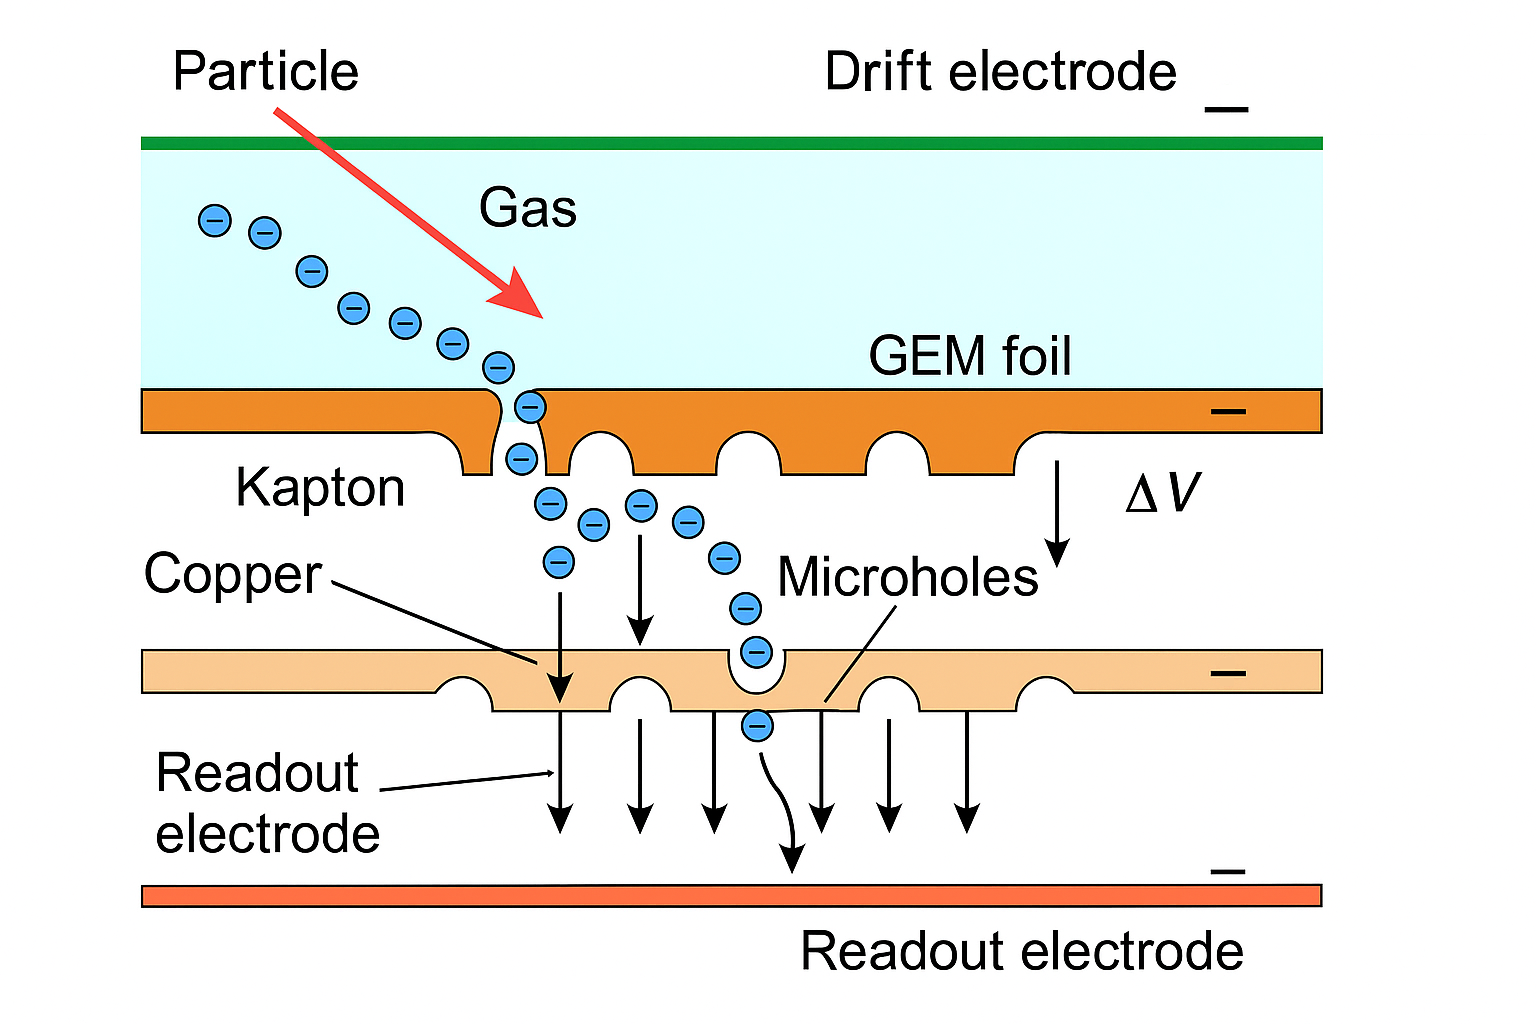
\includegraphics[width=0.5\textwidth, height=0.4\textwidth]{GEM}
\caption{Machine design}
\label{schema1}
\end{figure}

The electrons thus generated are subsequently accelerated by the electric fields present inside the detector, \ref{campo}, and passing through the microholes reach the photomultiplier tube.

\begin{figure}[H]
\centering
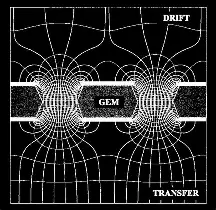
\includegraphics[width=0.4\textwidth, height=0.3\textwidth]{GEM4}
\caption{Electric field}
\label{campo}
\end{figure}

		\subsection{GEM}
			\subsubsection{What's a GEM?}
It's like a capacitor consisting of two layer of Copper (\ch{Cu}), that more easily we identify as top and bottom layer, fill between a layer of Kapton with size of 50$\mu$n. This foil has micrometric honeycomb-shaped biconical holes.

\begin{figure}[H]
\centering
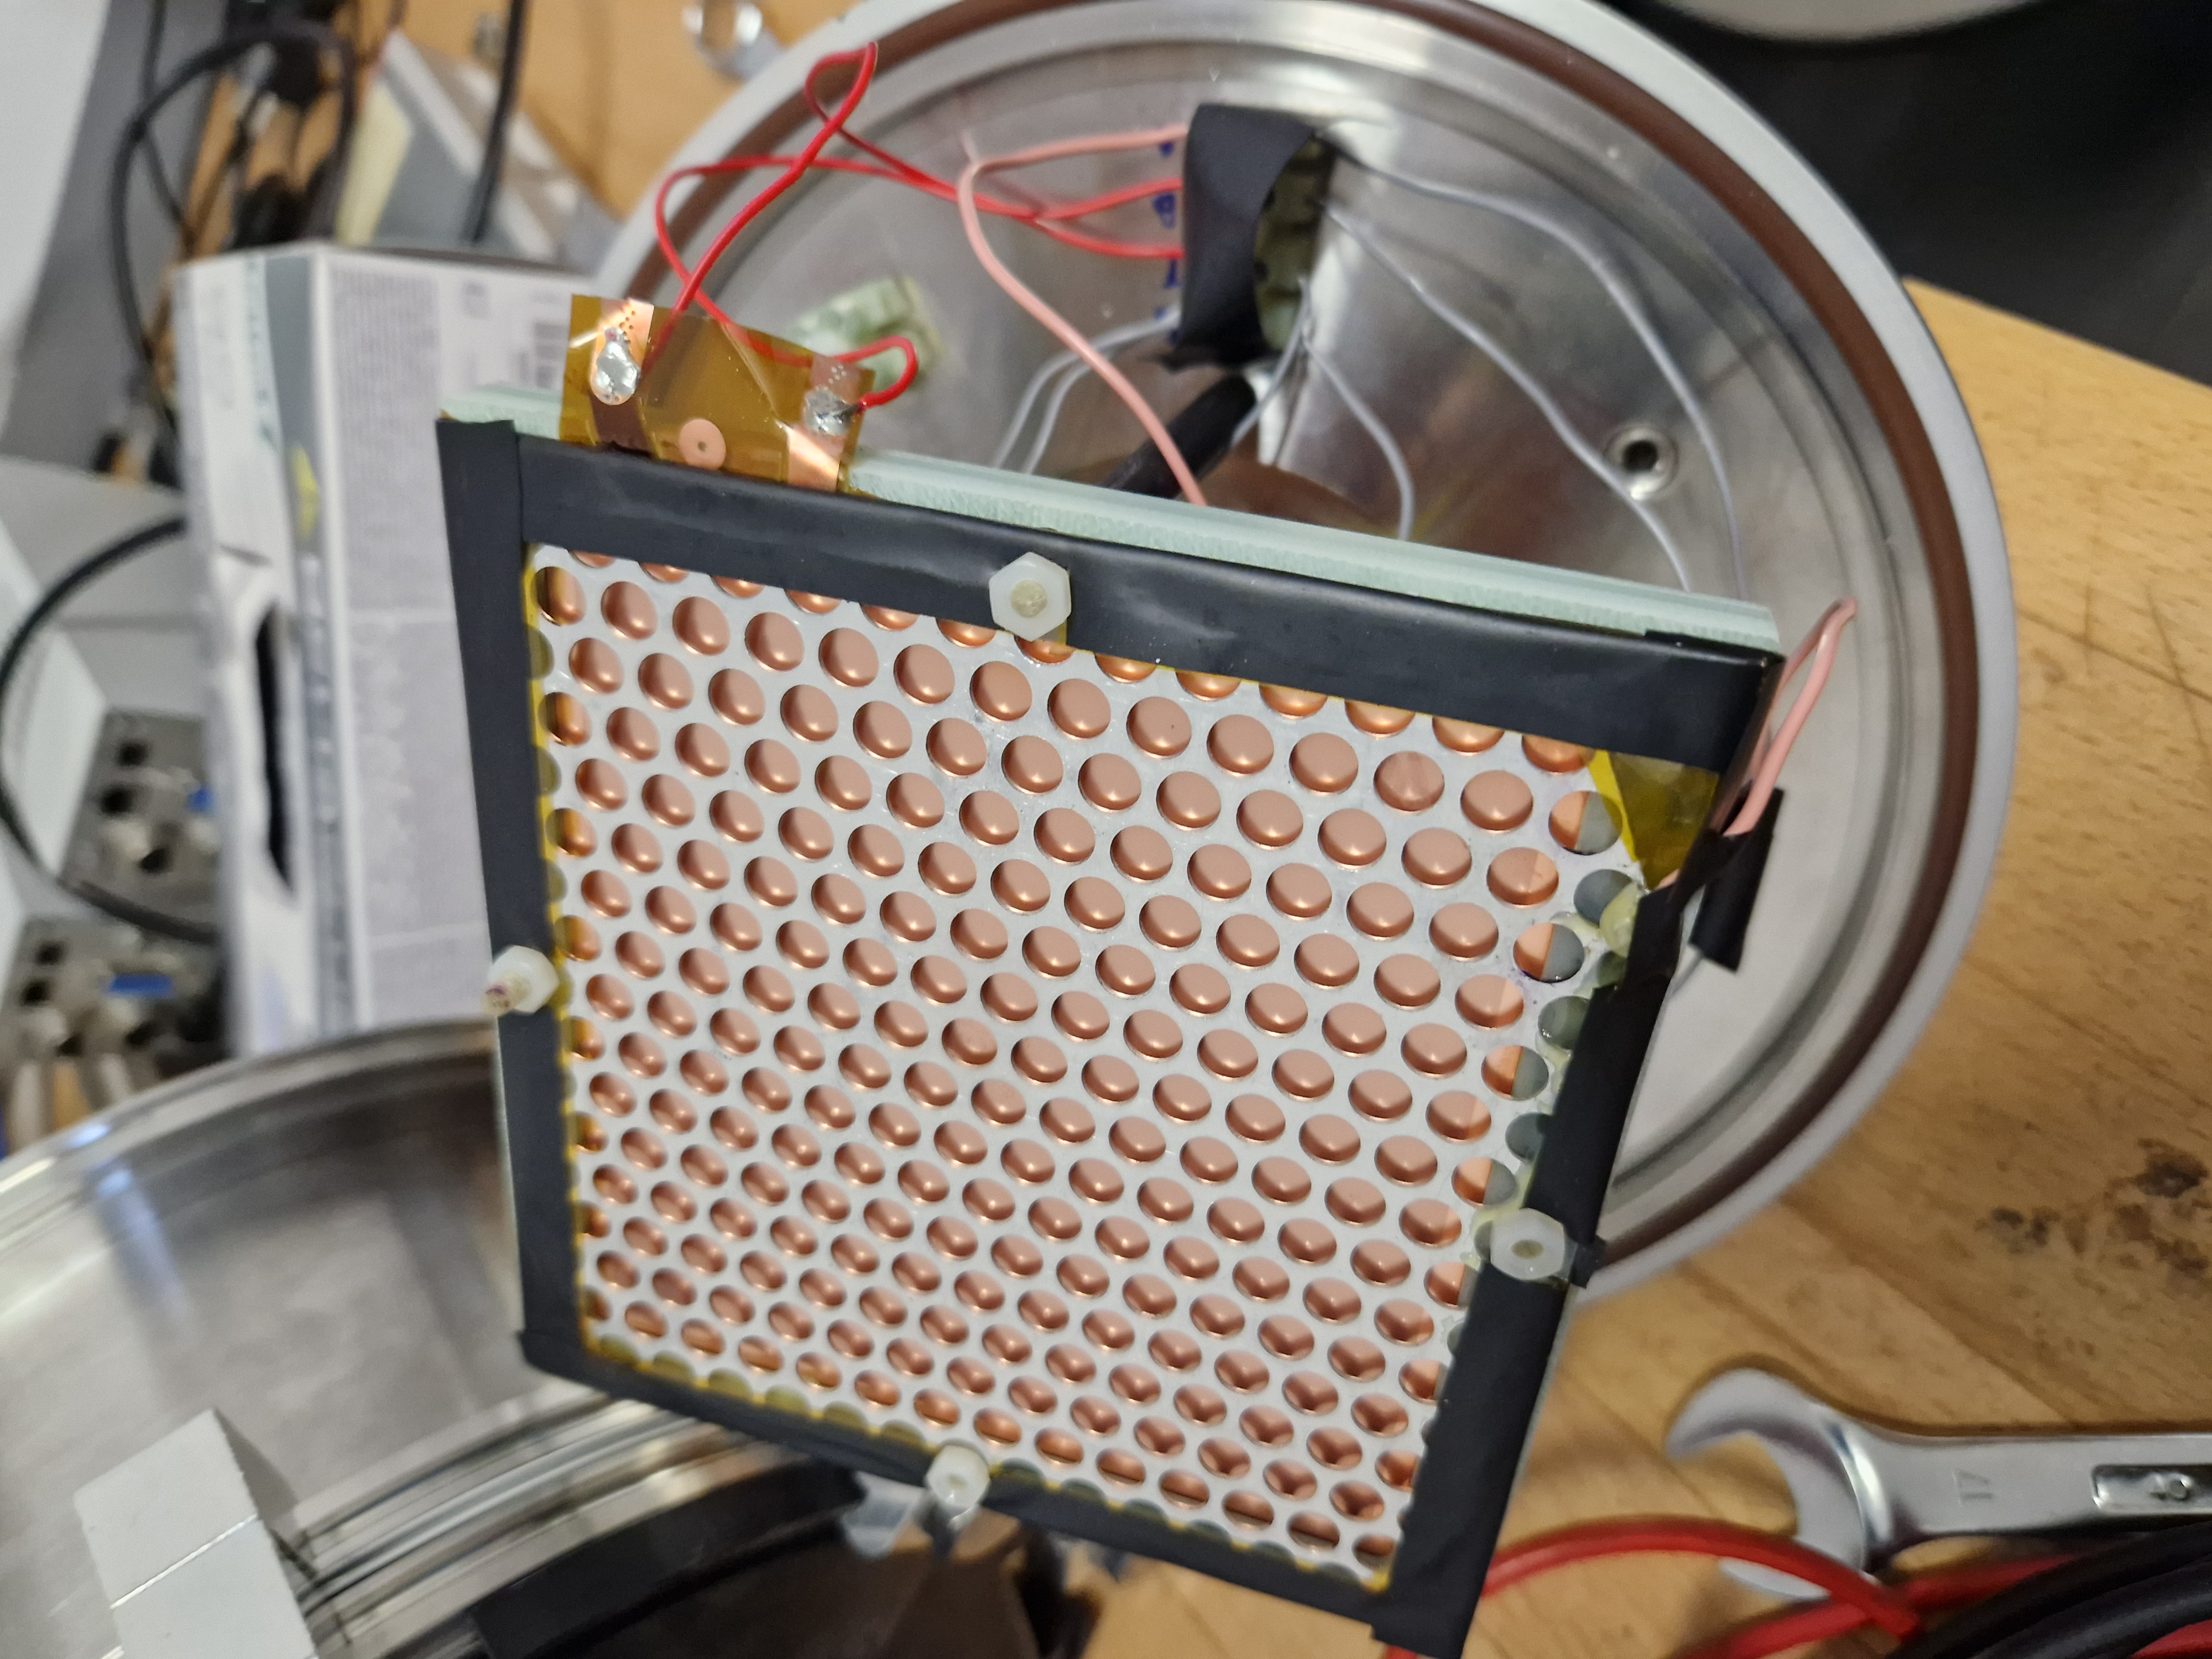
\includegraphics[width=0.4\textwidth, height=0.3\textwidth]{Griglia}
\caption{GEM in laboratory}
\end{figure}

The presence of micrometric holes allows to generate very strong electric fields in the holes to accelerate the electrons, furthermore the particular biconical shape prevents the formation of a discharge between top and bottom conductive layers.

\begin{figure}[H]
\centering
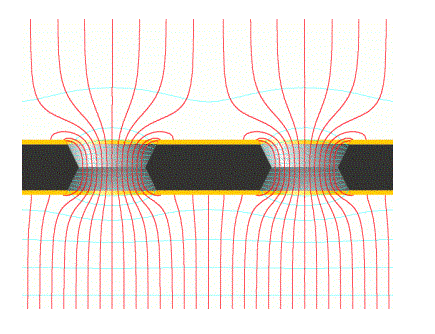
\includegraphics[width=0.4\textwidth, height=0.3\textwidth]{GEM6}
\caption{Micrometric biconical holes structure}
\end{figure}

			\subsubsection{Kapton}
Kapton is a polyimide film that is stable over a wide temperature range from -269 °C  up to +400 °C. It is the product of a condensation reaction between an aromatic diamine and pyromellitic anhydride.

\begin{figure}[H]
\centering
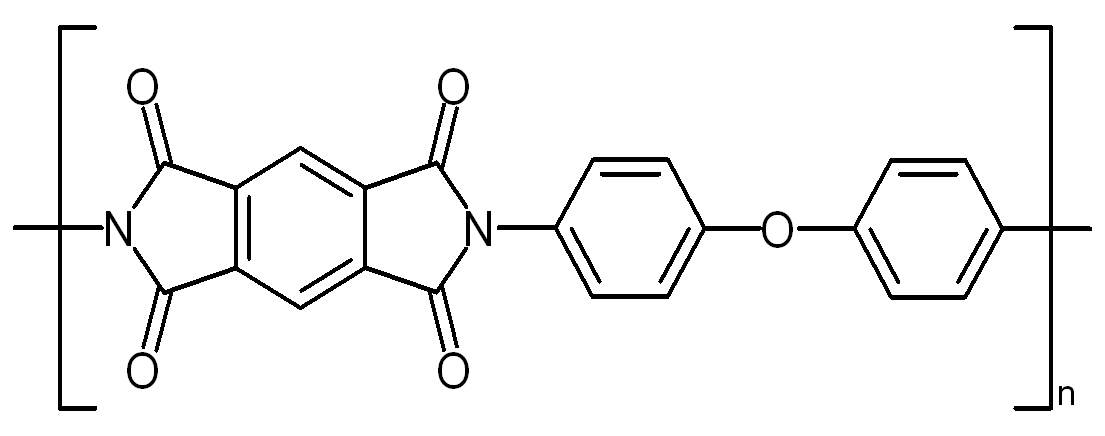
\includegraphics[width=0.4\textwidth, height=0.2\textwidth]{kapton}
\caption{Chemical formula of Kapton unit}
\end{figure}

			\subsubsection{Čerenkov effect}
The Čerenkov effect is the emission of electromagnetic radiation by a material, whose molecules are polarized by a charged particle moving through it. The emission of Čerenkov radiation occurs only when the speed of the particle moving through the environment is greater than the phase speed of light moving through the medium itself. More generally, we speak of Čerenkov radiation when the medium being crossed is not "transparent" to visible light.

This is due to the fact that the charged particle, along its trajectory, induces temporary dipole moments in the atoms or molecules of the environment. Returning to the initial configuration, the molecules produce electromagnetic radiation.\\

\textbf{Uses:} Čerenkov radiation is used primarily in scientific experiments involving the detection of particles of space origin. In immersion nuclear reactors, the intensity of the radiation is related to the frequency of fission events, and is therefore indicative of the level of activity of the reactor. Similarly, it is used to evaluate the residual radioactivity present in spent fuel rods.

		\subsection{PMT}
A PhotoMultiplier Tube is a electronic light detector in the ultraviolet and visible light. The device is so sensitive that it can detect a single photon. Therefore during the entire experience we have to cover the device with a thick blanket.

It consisting of a glass tube with a vacuum inside, containing an anode and several electrodes which constitute the dynodes, the operation of the photomultiplier is mainly based on two effects: the photoelectric effect and electromultiplication.

\begin{figure}[H]
\centering
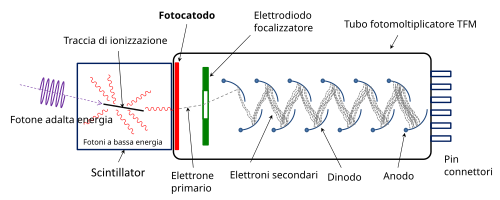
\includegraphics[width=0.5\textwidth, height=0.3\textwidth]{Schema PMT}
\caption{PMT scheme}
\end{figure}

The photons hit a photocathode through an input window, it's covered with a layer of material that promotes the photoelectric effect. Due to this effect the electrons are emitted and they are focused by an electrode towards the multiplication stage.

This stage consists of a series of electrodes, also call dynodes, each charged to a higher potential than the previous one. The first electron emitted by the photoelectric effect undergoes acceleration due to the electric field and acquires kinetic energy. When the electron hits the electrode corresponding to the first dynode, it causes the secondary emission of several electrons of lower energy. The structure of the system is designed so that each electron emitted by an electrode is accelerated and causes the emission of several electrons from the next electrode. This causes a cascade phenomenon where a single photon hitting the tube causes many electrons to pass through.

\begin{figure}[H]
\centering
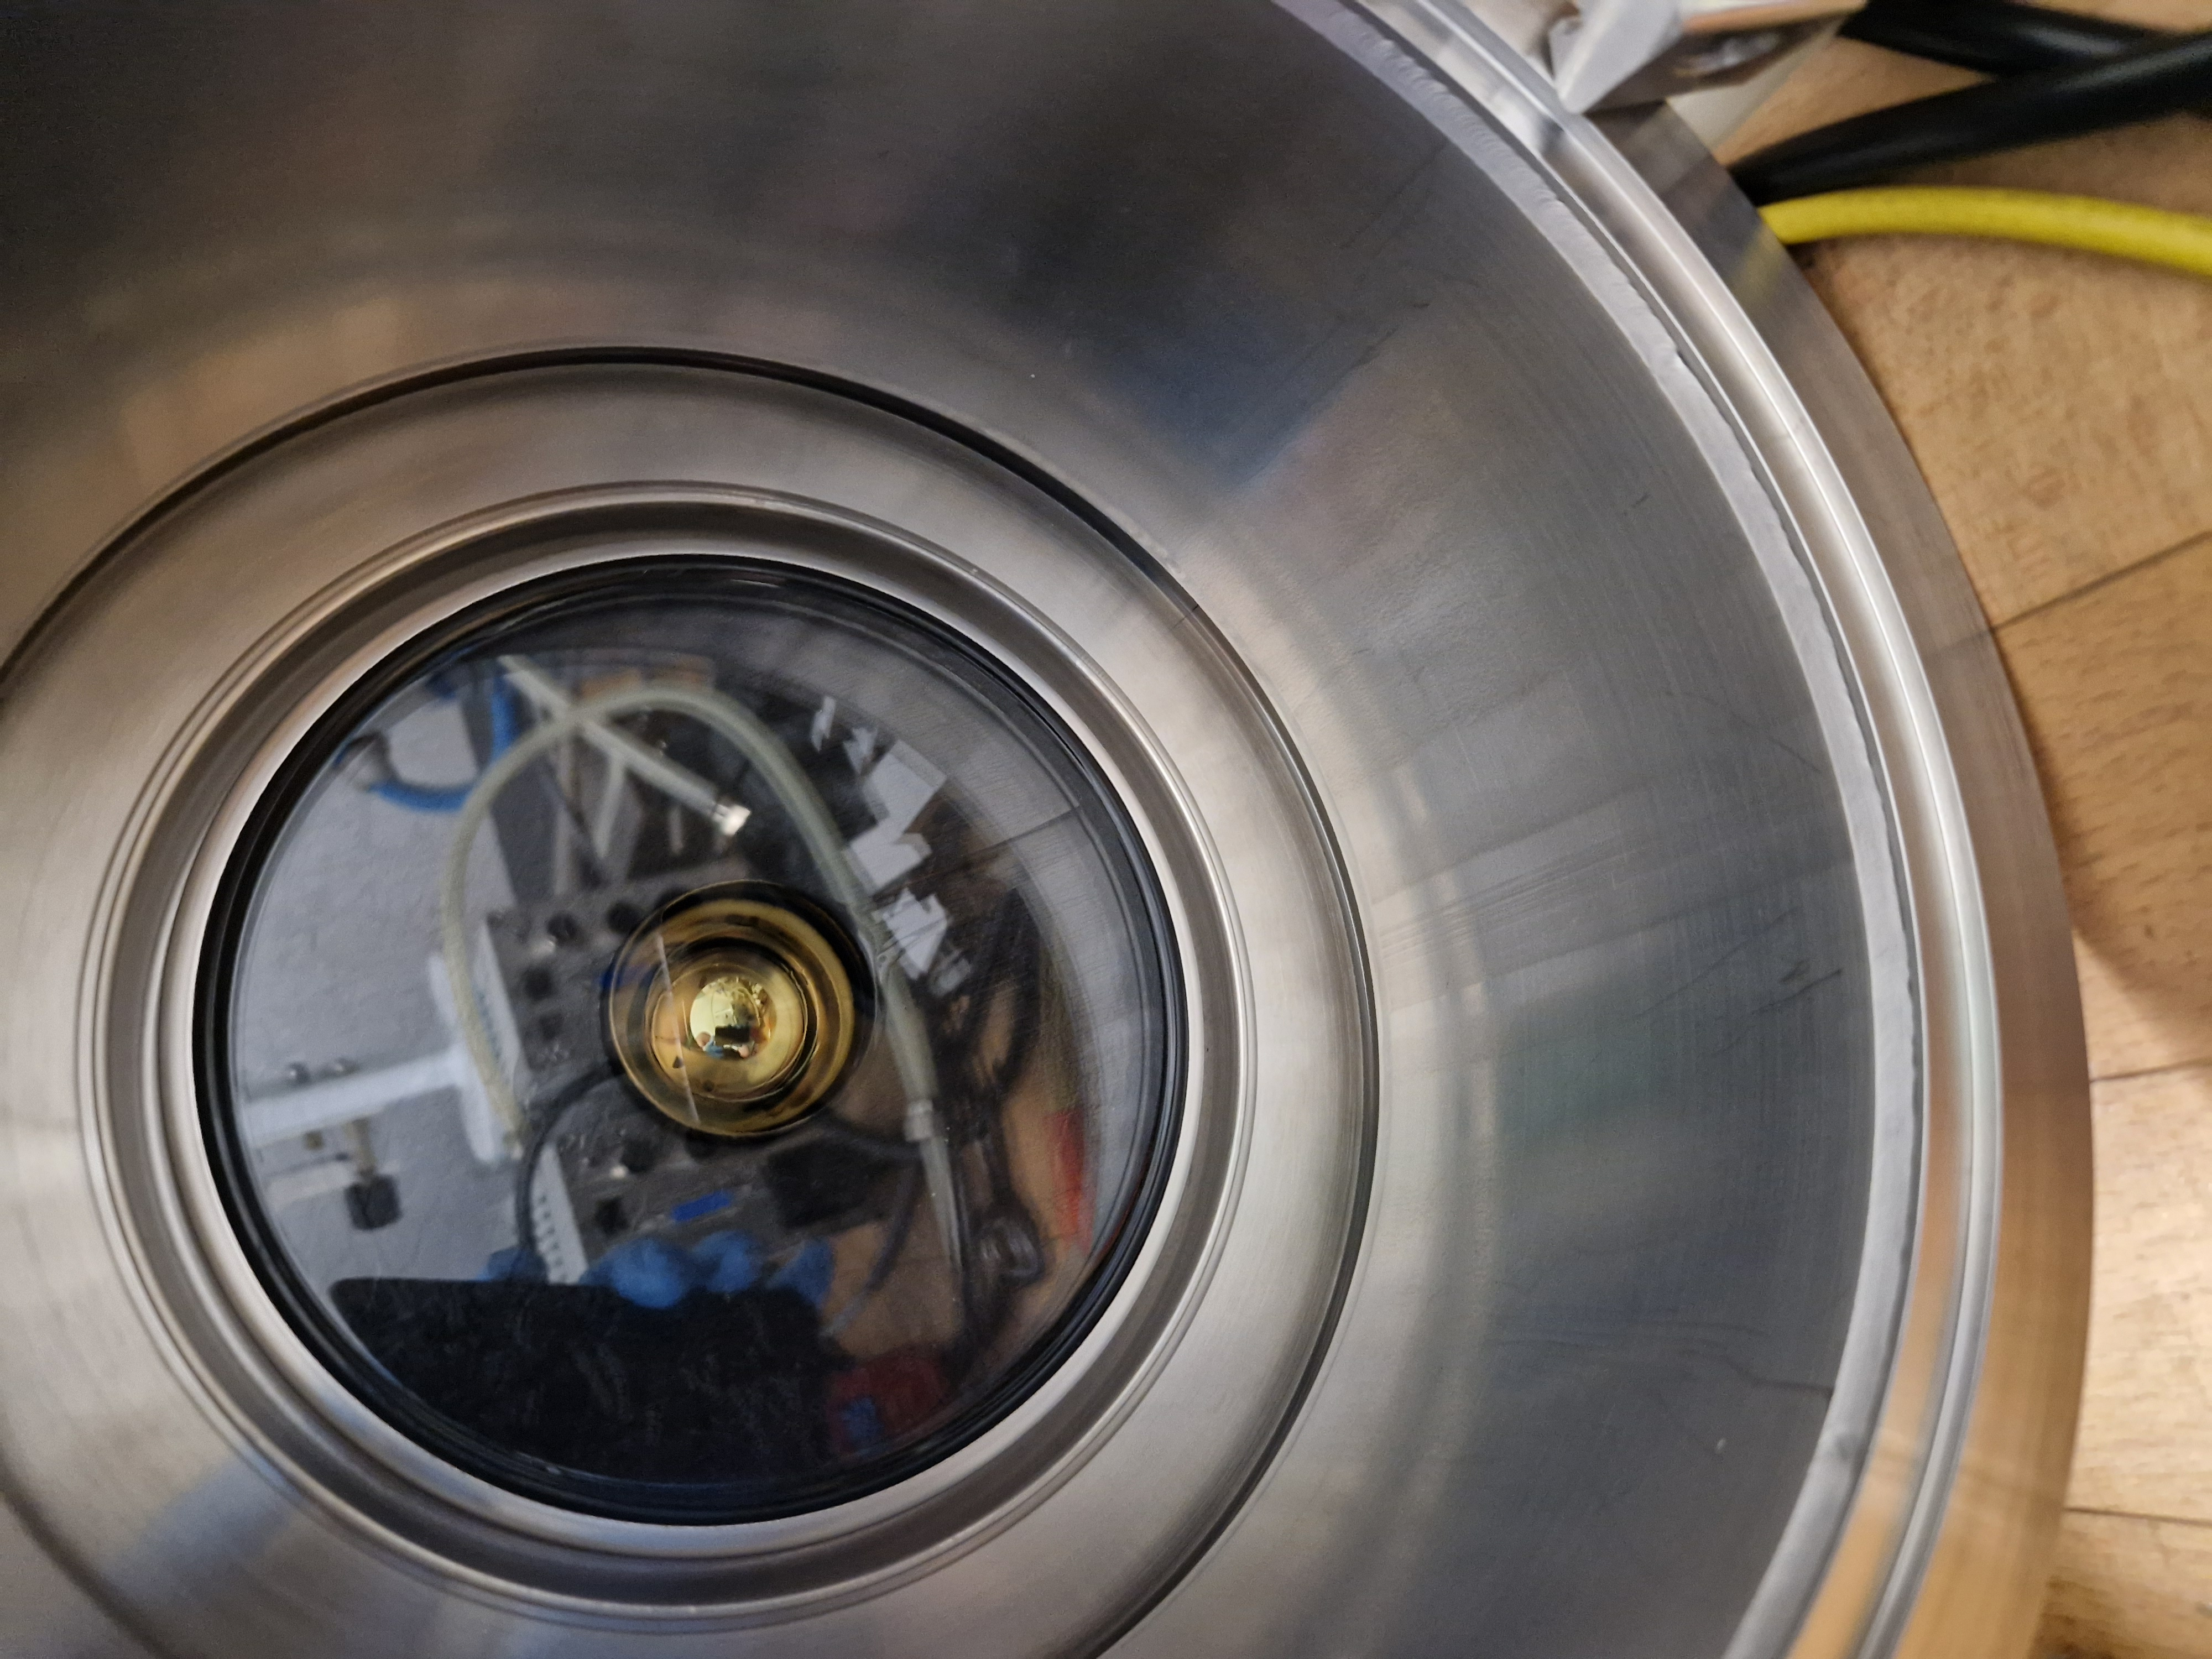
\includegraphics[width=0.4\textwidth, height=0.3\textwidth]{PMT1}
\caption{PMT in laboratory}
\end{figure}

	\section{Digitizer, RC circuit and Preamplifier}
About electrical components, in the experience we used a RC circuit between top and bottom of GEM, as it does not like too high current transients. So the circuit's main purpose is to cut and filter the high frequencies.

Instead, the preamplifier allows to amplify the signal without changing its shape (no shaping), since only a few photons reach the phototube. So the PMT will emit a small signal without the amplifier.

\chapter{Data Anlaysis}

\begin{figure}[H]
\centering
\rotatebox{270}{%
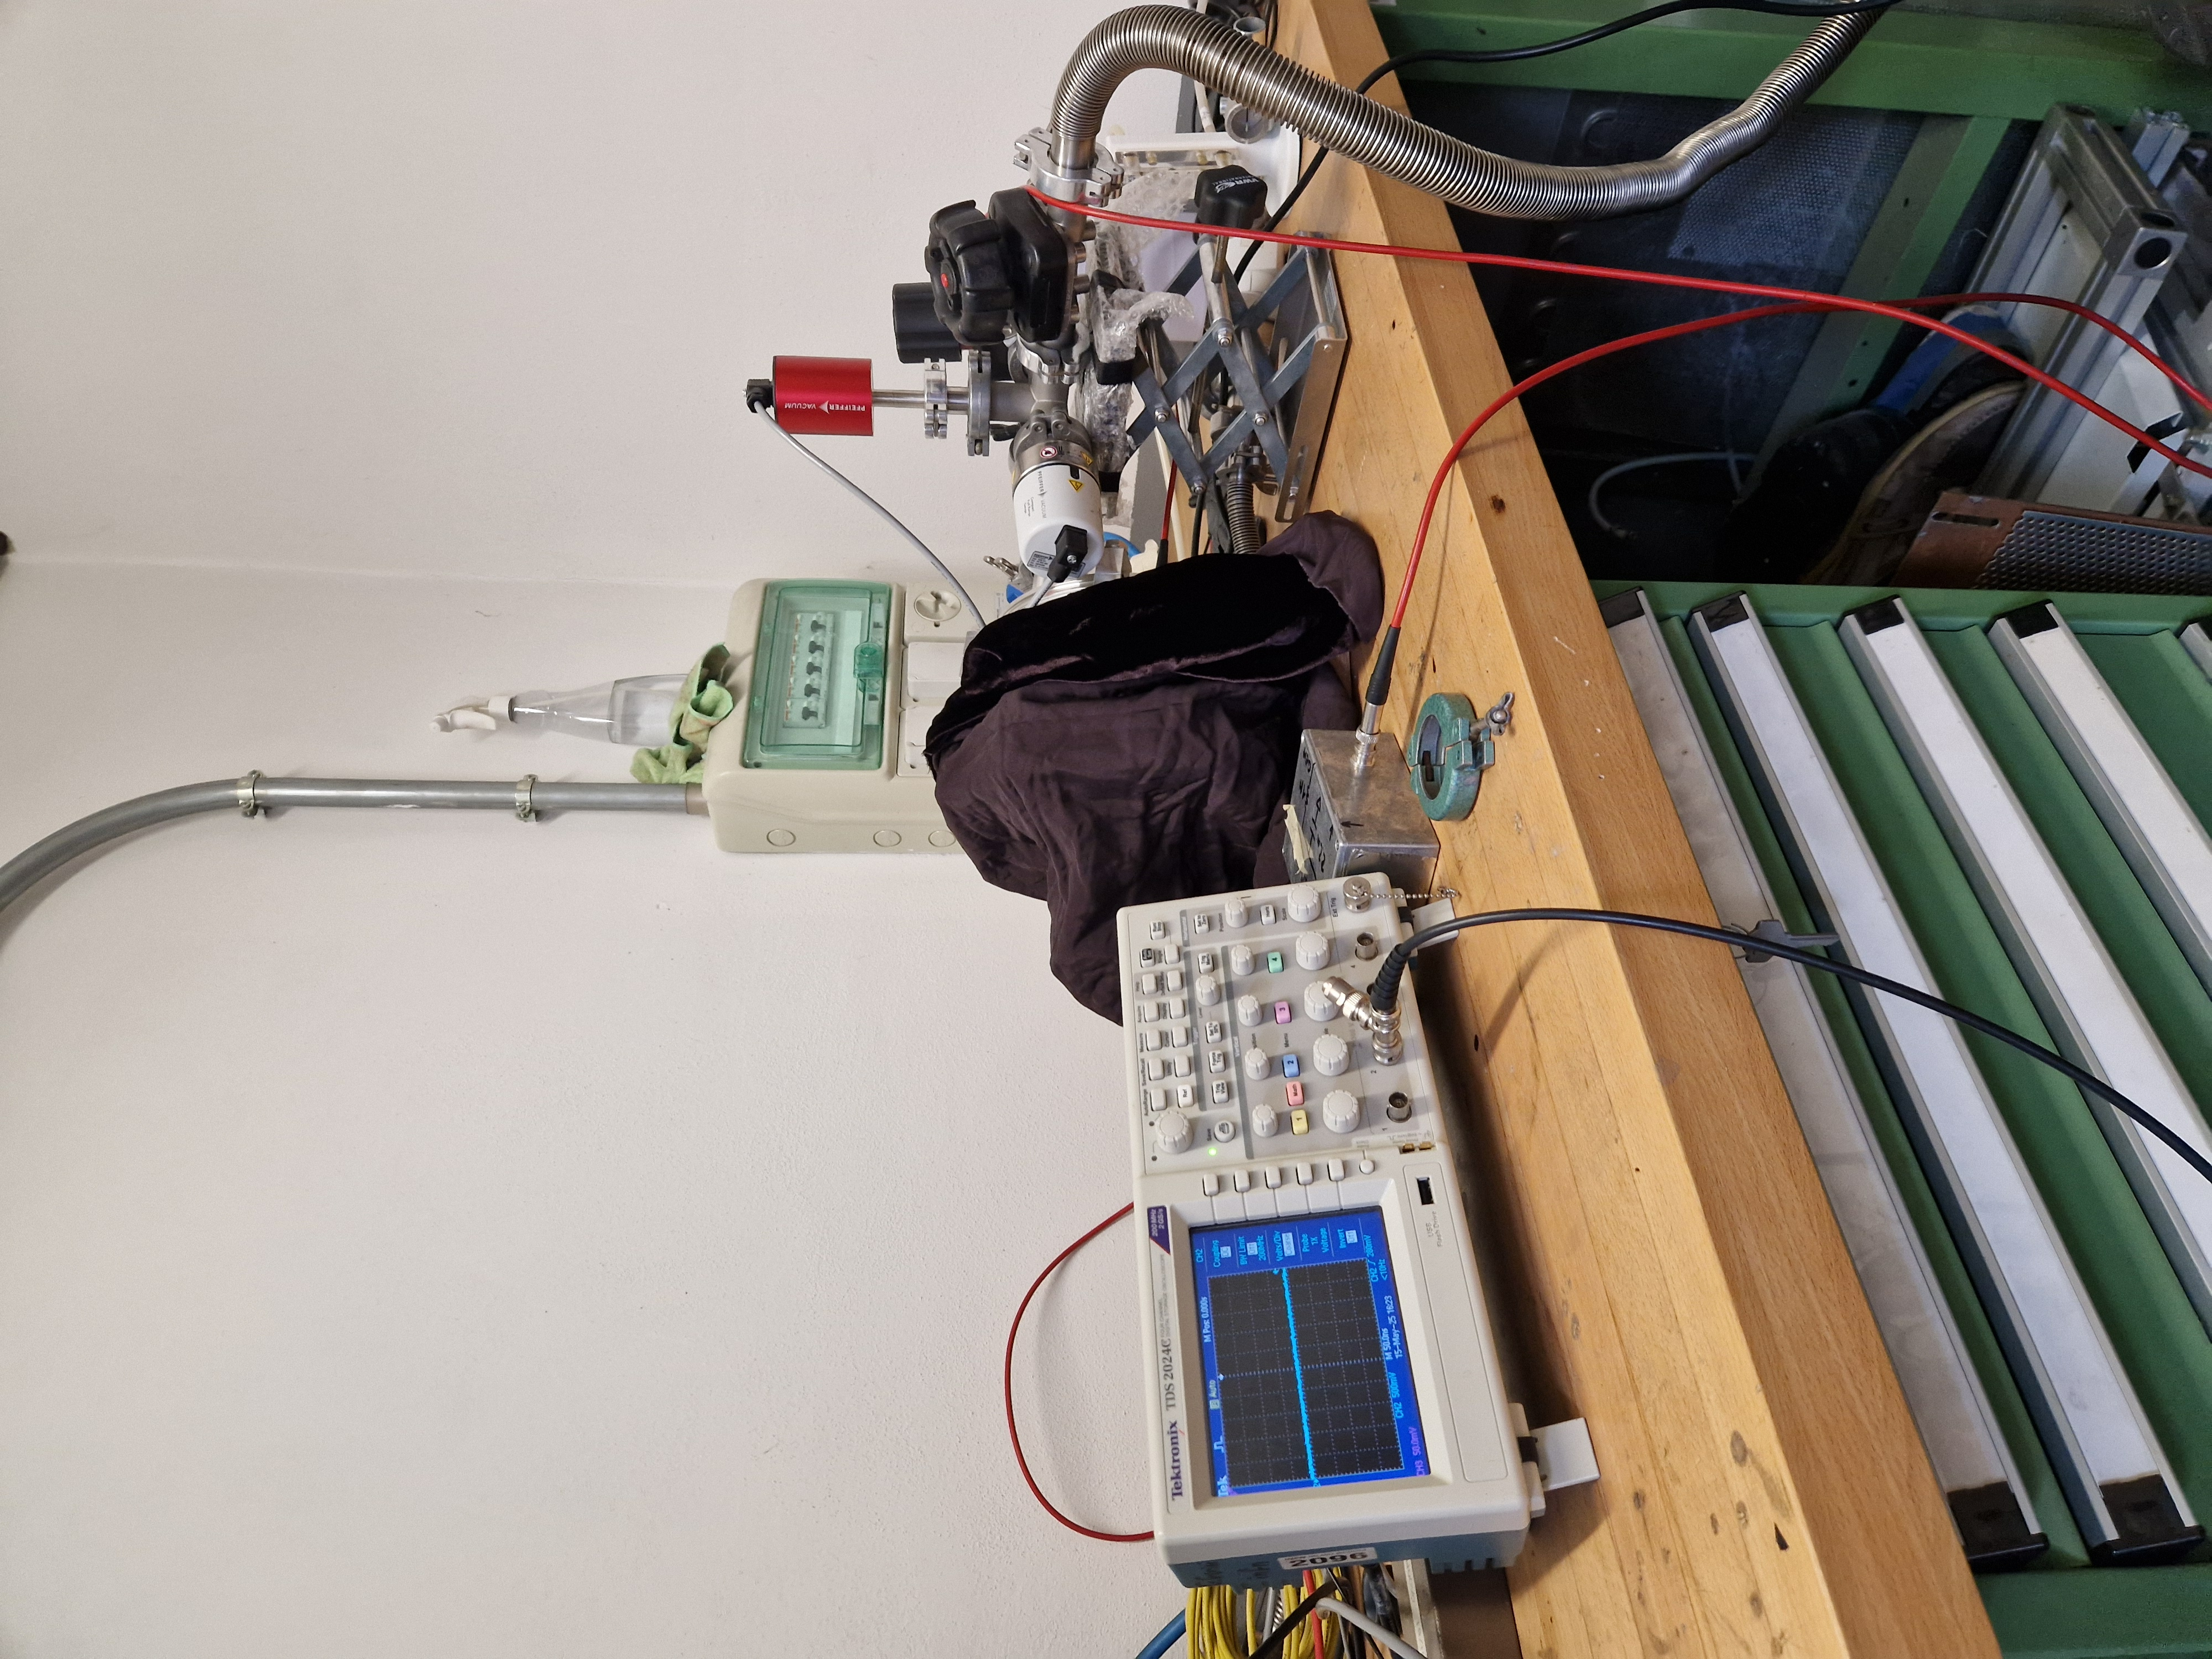
\includegraphics[width=0.5\textwidth, height=0.4\textwidth]{Setup}}
\caption{Setup sperimentale}
\end{figure}

For the analysis we developed a program able to read the duration of the signal beyond a certain threshold.

The operating principle is based on the search for minimums beyond a certain threshold, chosen by calculating a horizontal line averaging the values obtained in the dataset and the relative standard deviation.

Once the data set has been decreased, the start and end peaks are searched for using an ad hoc generated algorithm, thus defining whether the signal being analyzed is a good signal or a bad one. Starting from the first peak present, an interval of values $\pm100$ is detached that entered on the current minimum. If another peak is identified in the interval thus defined, the operation is iterated until the last peak that satisfies the conditions is identified. If, however, there are no further peaks or single peaks in the interval, then this is defined as bad.

During the analysis according to the algorithm defined in this way we found some cases not correctly managed, mainly caused by the electronic noise of the instrumentation that does not allow the correct analysis of all the counts. We therefore estimated 1/10 counts not managed.

Finally there are cases of electronic noise that however fall within or at least slightly lengthen the signal as in figure \ref{lungo}.
\begin{figure}[H]
\centering
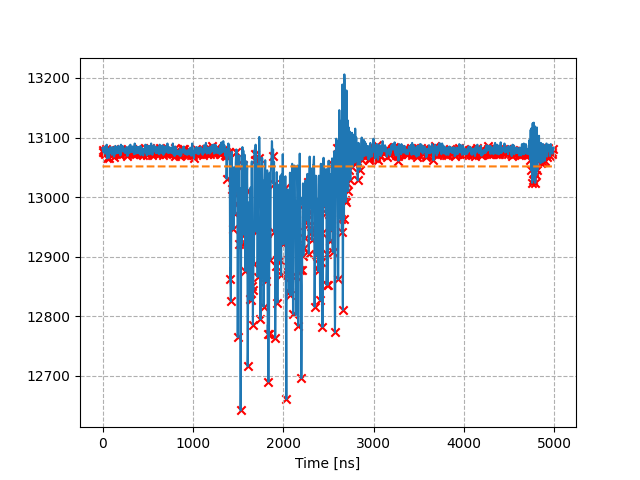
\includegraphics[width=0.4\textwidth, height=0.3\textwidth]{Bad_rumore4}
\caption{Elongated signal}
\label{lungo}
\end{figure}

		\subsection{Good Count}
Here we show some example of good signal:
\begin{figure}[H]
\centering
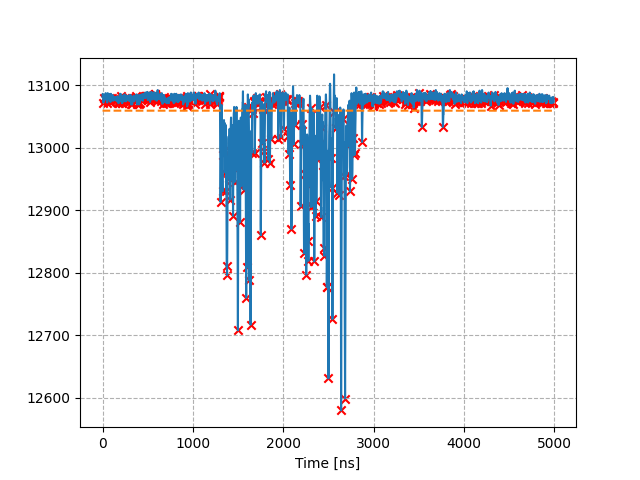
\includegraphics[width=0.4\textwidth, height=0.3\textwidth]{Buona}
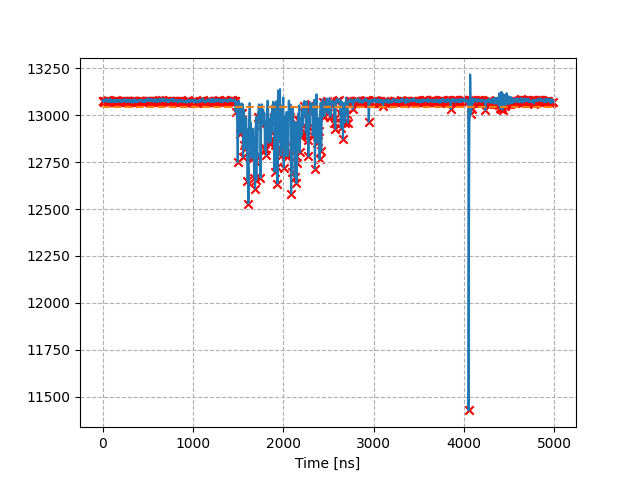
\includegraphics[width=0.4\textwidth, height=0.3\textwidth]{Buona2}
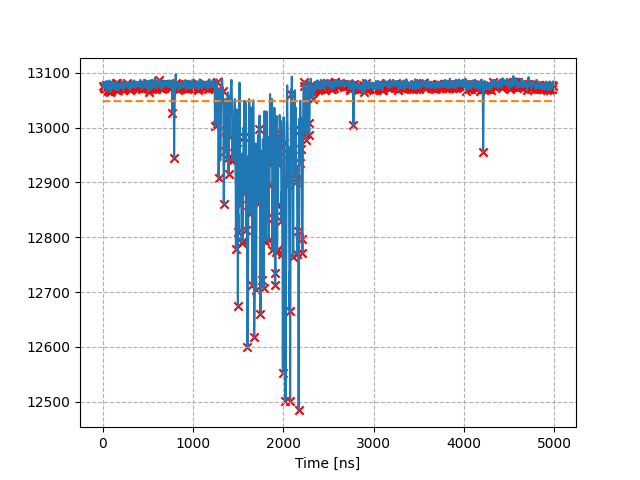
\includegraphics[width=0.4\textwidth, height=0.3\textwidth]{Buona3}
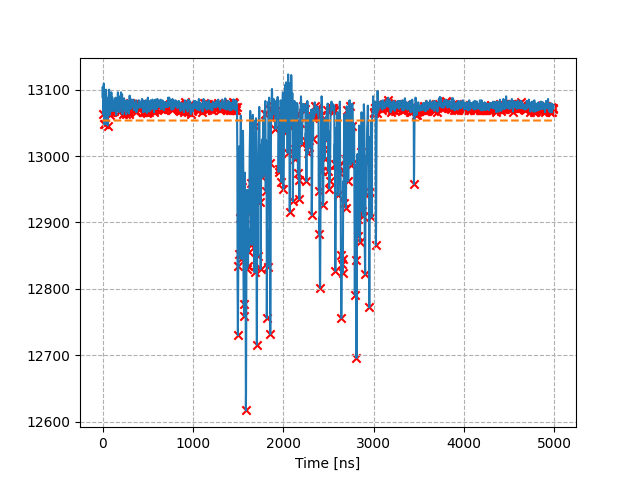
\includegraphics[width=0.4\textwidth, height=0.3\textwidth]{Buona4}
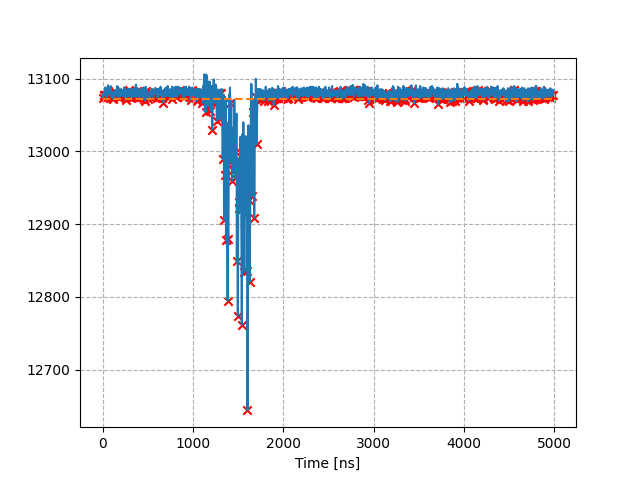
\includegraphics[width=0.4\textwidth, height=0.3\textwidth]{Buona5}
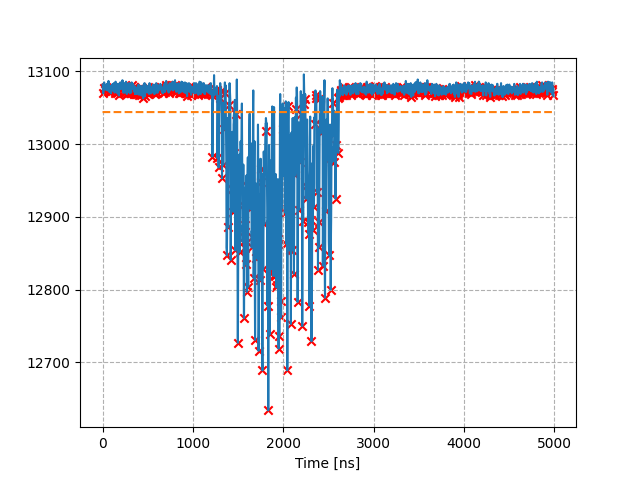
\includegraphics[width=0.4\textwidth, height=0.3\textwidth]{Buona6}
\caption{Good count}
\end{figure}

Good count correctly handled, the algorithm can distinguish noise in this case because it comes after the signal.
\begin{figure}[H]
\centering
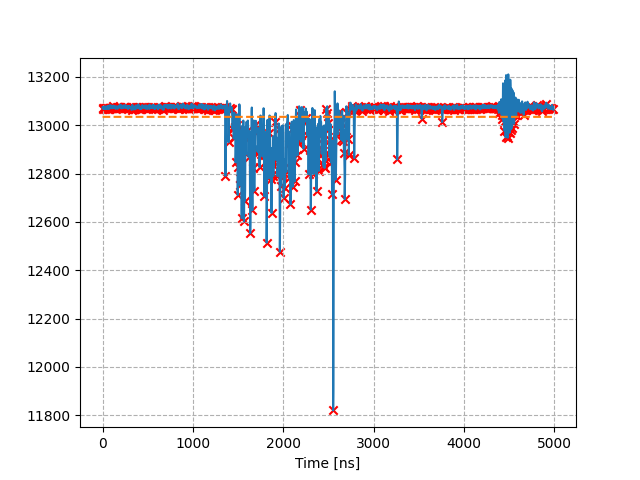
\includegraphics[width=0.4\textwidth, height=0.3\textwidth]{All}
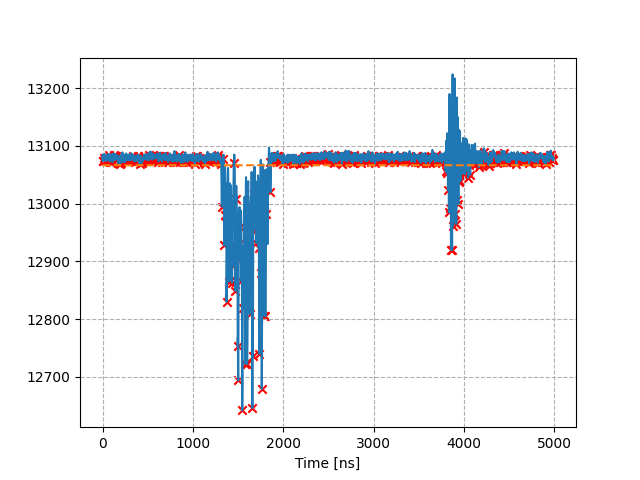
\includegraphics[width=0.4\textwidth, height=0.3\textwidth]{Bad_rumore2}
\caption{Good count with noise}
\end{figure}

		\subsection{Bad Count}
Bad count correctly handled:
\begin{figure}[H]
\centering
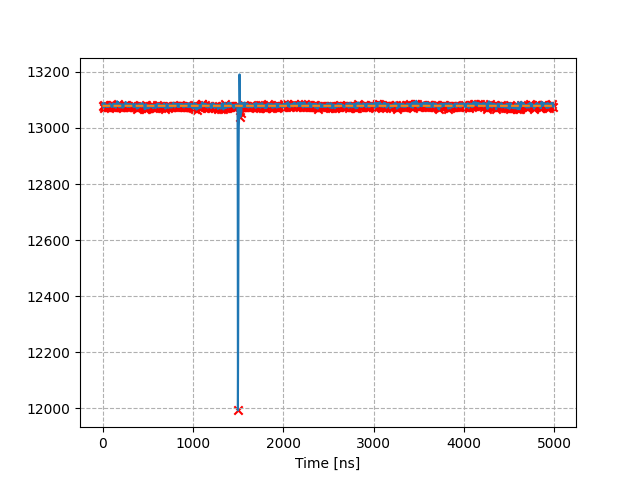
\includegraphics[width=0.4\textwidth, height=0.3\textwidth]{Bad}
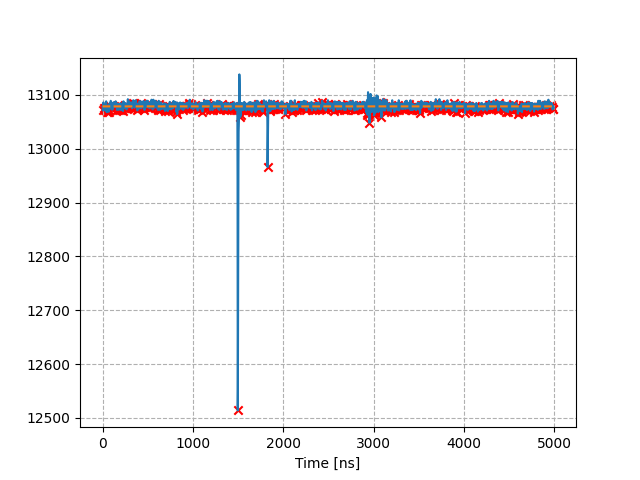
\includegraphics[width=0.4\textwidth, height=0.3\textwidth]{Bad2}
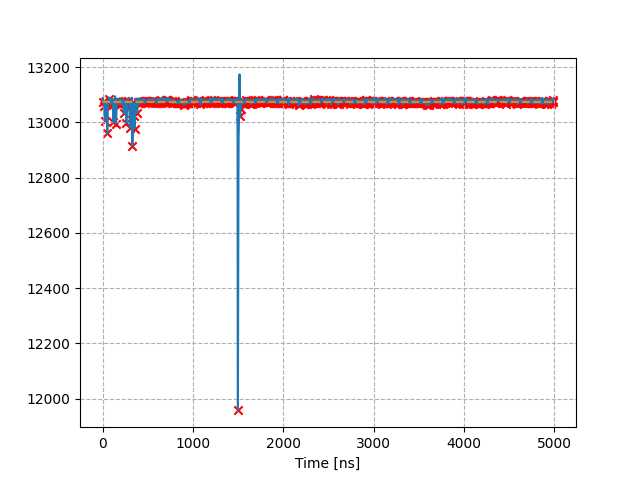
\includegraphics[width=0.4\textwidth, height=0.3\textwidth]{Bad3}
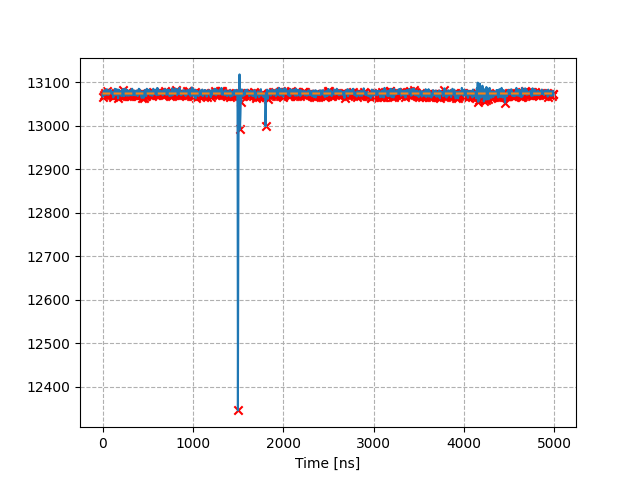
\includegraphics[width=0.4\textwidth, height=0.3\textwidth]{Bad4}
\caption{Bad count handled}
\end{figure}

Bad count not handled because the noise come before the signal.
\begin{figure}[H]
\centering
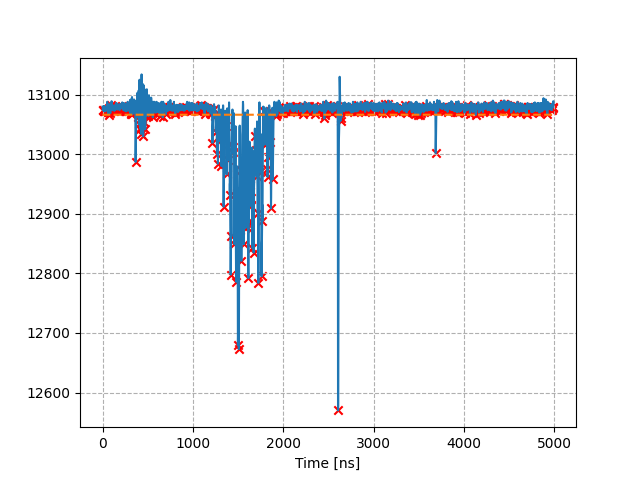
\includegraphics[width=0.4\textwidth, height=0.3\textwidth]{Bad_rumore}
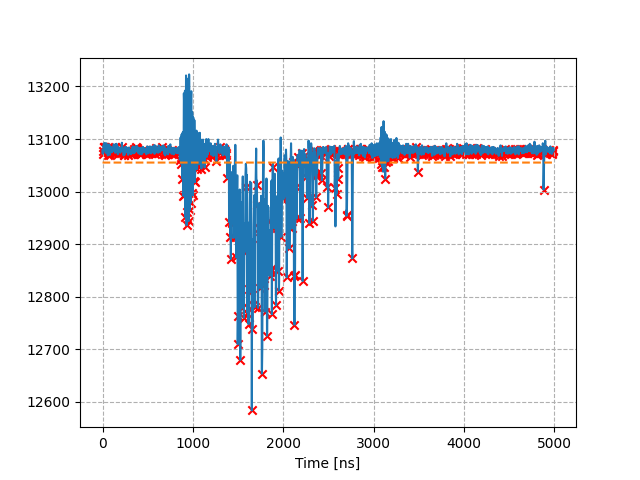
\includegraphics[width=0.4\textwidth, height=0.3\textwidth]{Bad_rumore3}
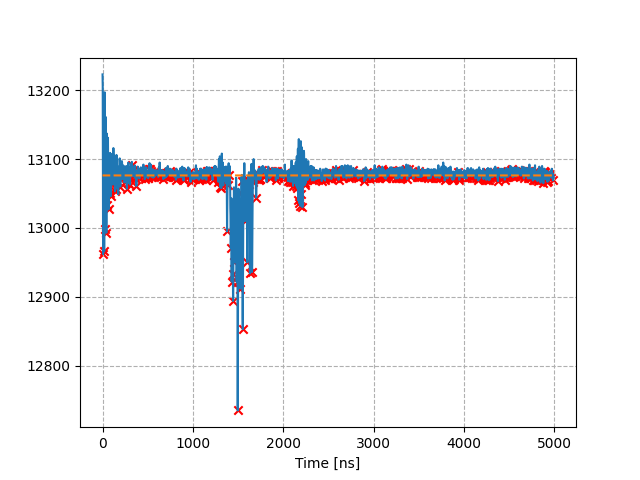
\includegraphics[width=0.4\textwidth, height=0.3\textwidth]{Doppio_bad2}
\caption{Bad count not handled}
\end{figure}

	\section{Drift Range}
In this section we changed the voltage difference present between the cathode and the top's GEM in according whit the parameters in table \ref{driftrange}
\begin{table}[H]
\centering
\begin{tabular}{l|c|c|c|c}\hline
\textbf{File}&\textbf{Cathode [V]}&\textbf{Top GEM [V]}&\textbf{Bottom GEM [V]}&\textbf{PMT [V]}\\
drift10&2999.8&499.6&100.8&1400.8\\\hline
drift9&2799.8&499.6&100.8&1400.8\\\hline
drift8&2499.8&499.6&100.8&1400.8\\\hline
drift7&2250&499.6&100.8&1400.8\\\hline
drift6&2000&499.6&100.8&1400.8\\\hline
drift5&1750&499.6&100.8&1400.8\\\hline
drift4&1500&499.6&100.8&1400.8\\\hline
drift3&1250.2&499.6&100.8&1400.8\\\hline
drift2&1000.4&499.6&100.8&1400.8\\\hline
drift1&750.6&499.6&100.8&1400.8\\\hline
\end{tabular}
\caption{Voltage parameters}
\label{driftrange}
\end{table}

By changing cathode voltage we observed an increased average signal duration which translates into more energetic particles.

\begin{figure}[H]
\centering
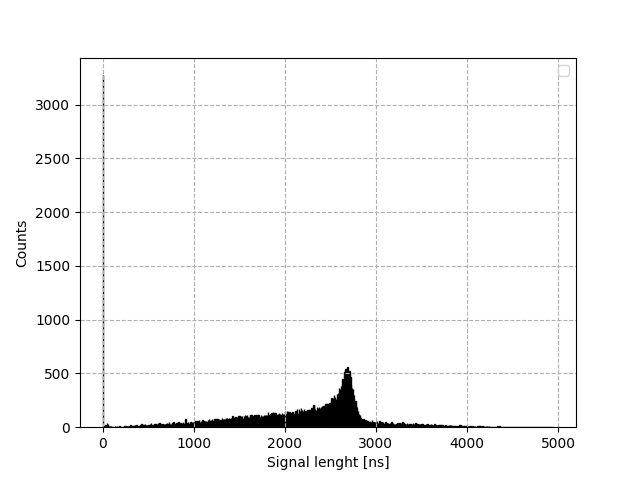
\includegraphics[width=0.4\textwidth, height=0.3\textwidth]{Histo_drift1}
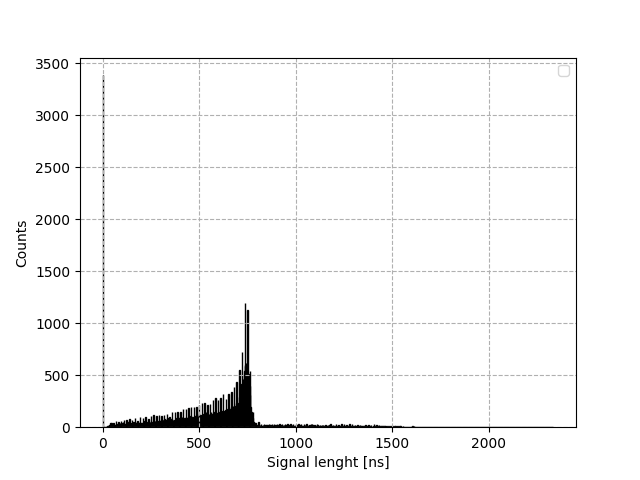
\includegraphics[width=0.4\textwidth, height=0.3\textwidth]{Histo_drift10}
\caption{From Drift1 to Drift10}
\end{figure}

\begin{figure}[H]
\centering
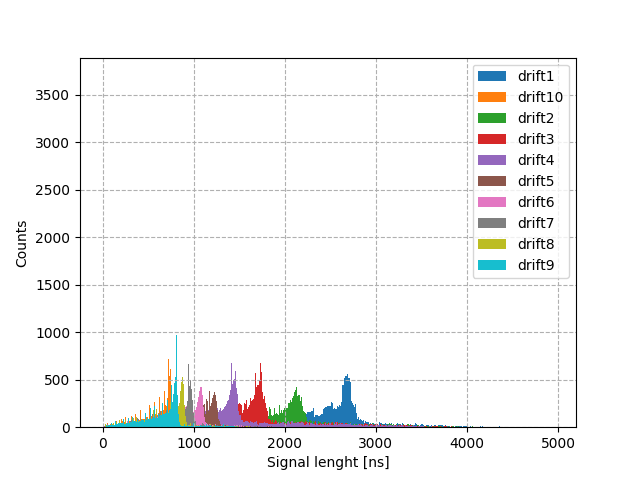
\includegraphics[width=0.5\textwidth, height=0.4\textwidth]{Histo_drift}
\caption{Changing in drift stage}
\end{figure}

	\section{Top Range}
Meanwhile in this section we changed the voltage difference present between the top's GEM and the bottom's GEM in according whit the parameters in table \ref{toprange}
\begin{table}[H]
\centering
\begin{tabular}{l|c|c|c|c}\hline
\textbf{File}&\textbf{Cathode [V]}&\textbf{Top GEM [V]}&\textbf{Bottom GEM [V]}&\textbf{PMT [V]}\\
top1&850.4&599.8&100.8&1400.8\\\hline
top2&800.2&549.8&100.8&1400.8\\\hline
top3&750.4&499.6&100.8&1400.8\\\hline
top4&700.2&449.6&100.8&1400.8\\\hline
top5&650.2&399.4&100.8&1400.8\\\hline
top6&600.4&349.6&100.8&1400.8\\\hline
\end{tabular}
\caption{Voltage parameters}
\label{toprange}
\end{table}

At low voltages the signal duration is very dispersive, while by increasing the voltage the duration stabilizes around 2700 ns

\begin{figure}[H]
\centering
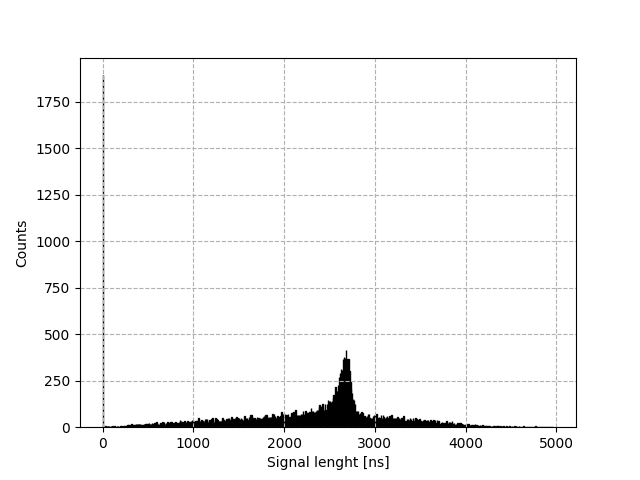
\includegraphics[width=0.4\textwidth, height=0.3\textwidth]{Histo_top1}
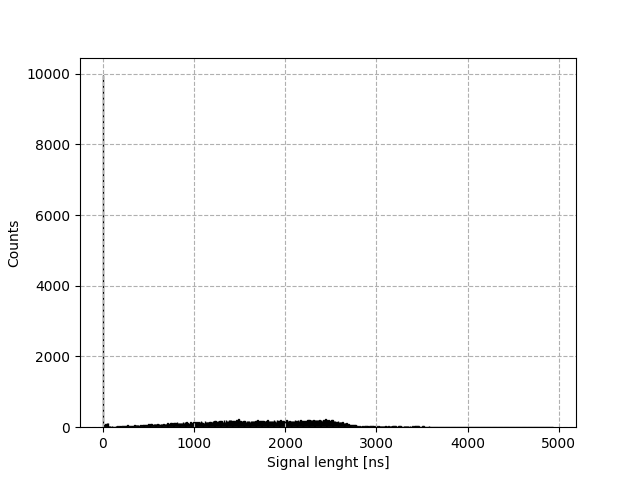
\includegraphics[width=0.4\textwidth, height=0.3\textwidth]{Histo_top6}
\caption{From Top1 to Top6}
\end{figure}

\begin{figure}[H]
\centering
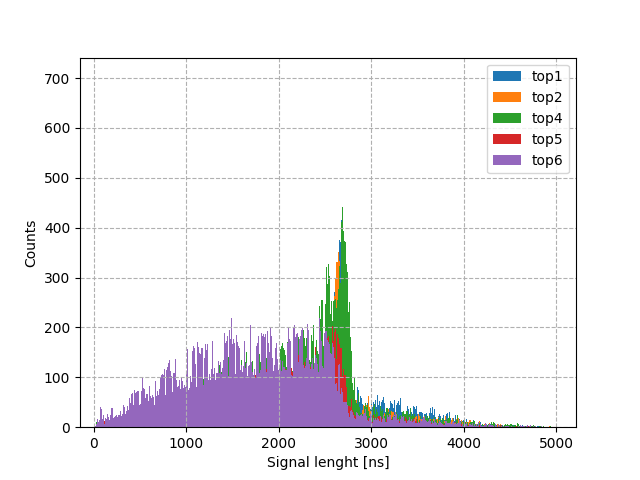
\includegraphics[width=0.5\textwidth, height=0.4\textwidth]{Histo_top}
\caption{Changing in top stage}
\end{figure}
\end{document}